\hypertarget{section-concepts}{%
\section{Cross-cutting Concepts}\label{section-concepts}}

\subsection{Centralized Authentication}

Authentication ensures secure access to the Escape Doom system using an external provider (Keycloak) to manage user identities. OAuth ensures secure communication through short-lived access tokens and the API Gateway acts as a central entry point for all requests, ensuring validation of access tokens and enforces access control across microservices.

\begin{enumerate}
    \item A user submits credentials to Keycloak via the OAuth authorization flow.
    \item Keycloak authenticates the user and issues an OAuth access token. The access token is included in all API requests.
    \item The API Gateway validates the access token against Keycloak and enforces access control.
    \item Requests that pass validation are routed to backend microservices.
\end{enumerate}

\begin{figure}[h!]
    \centering
    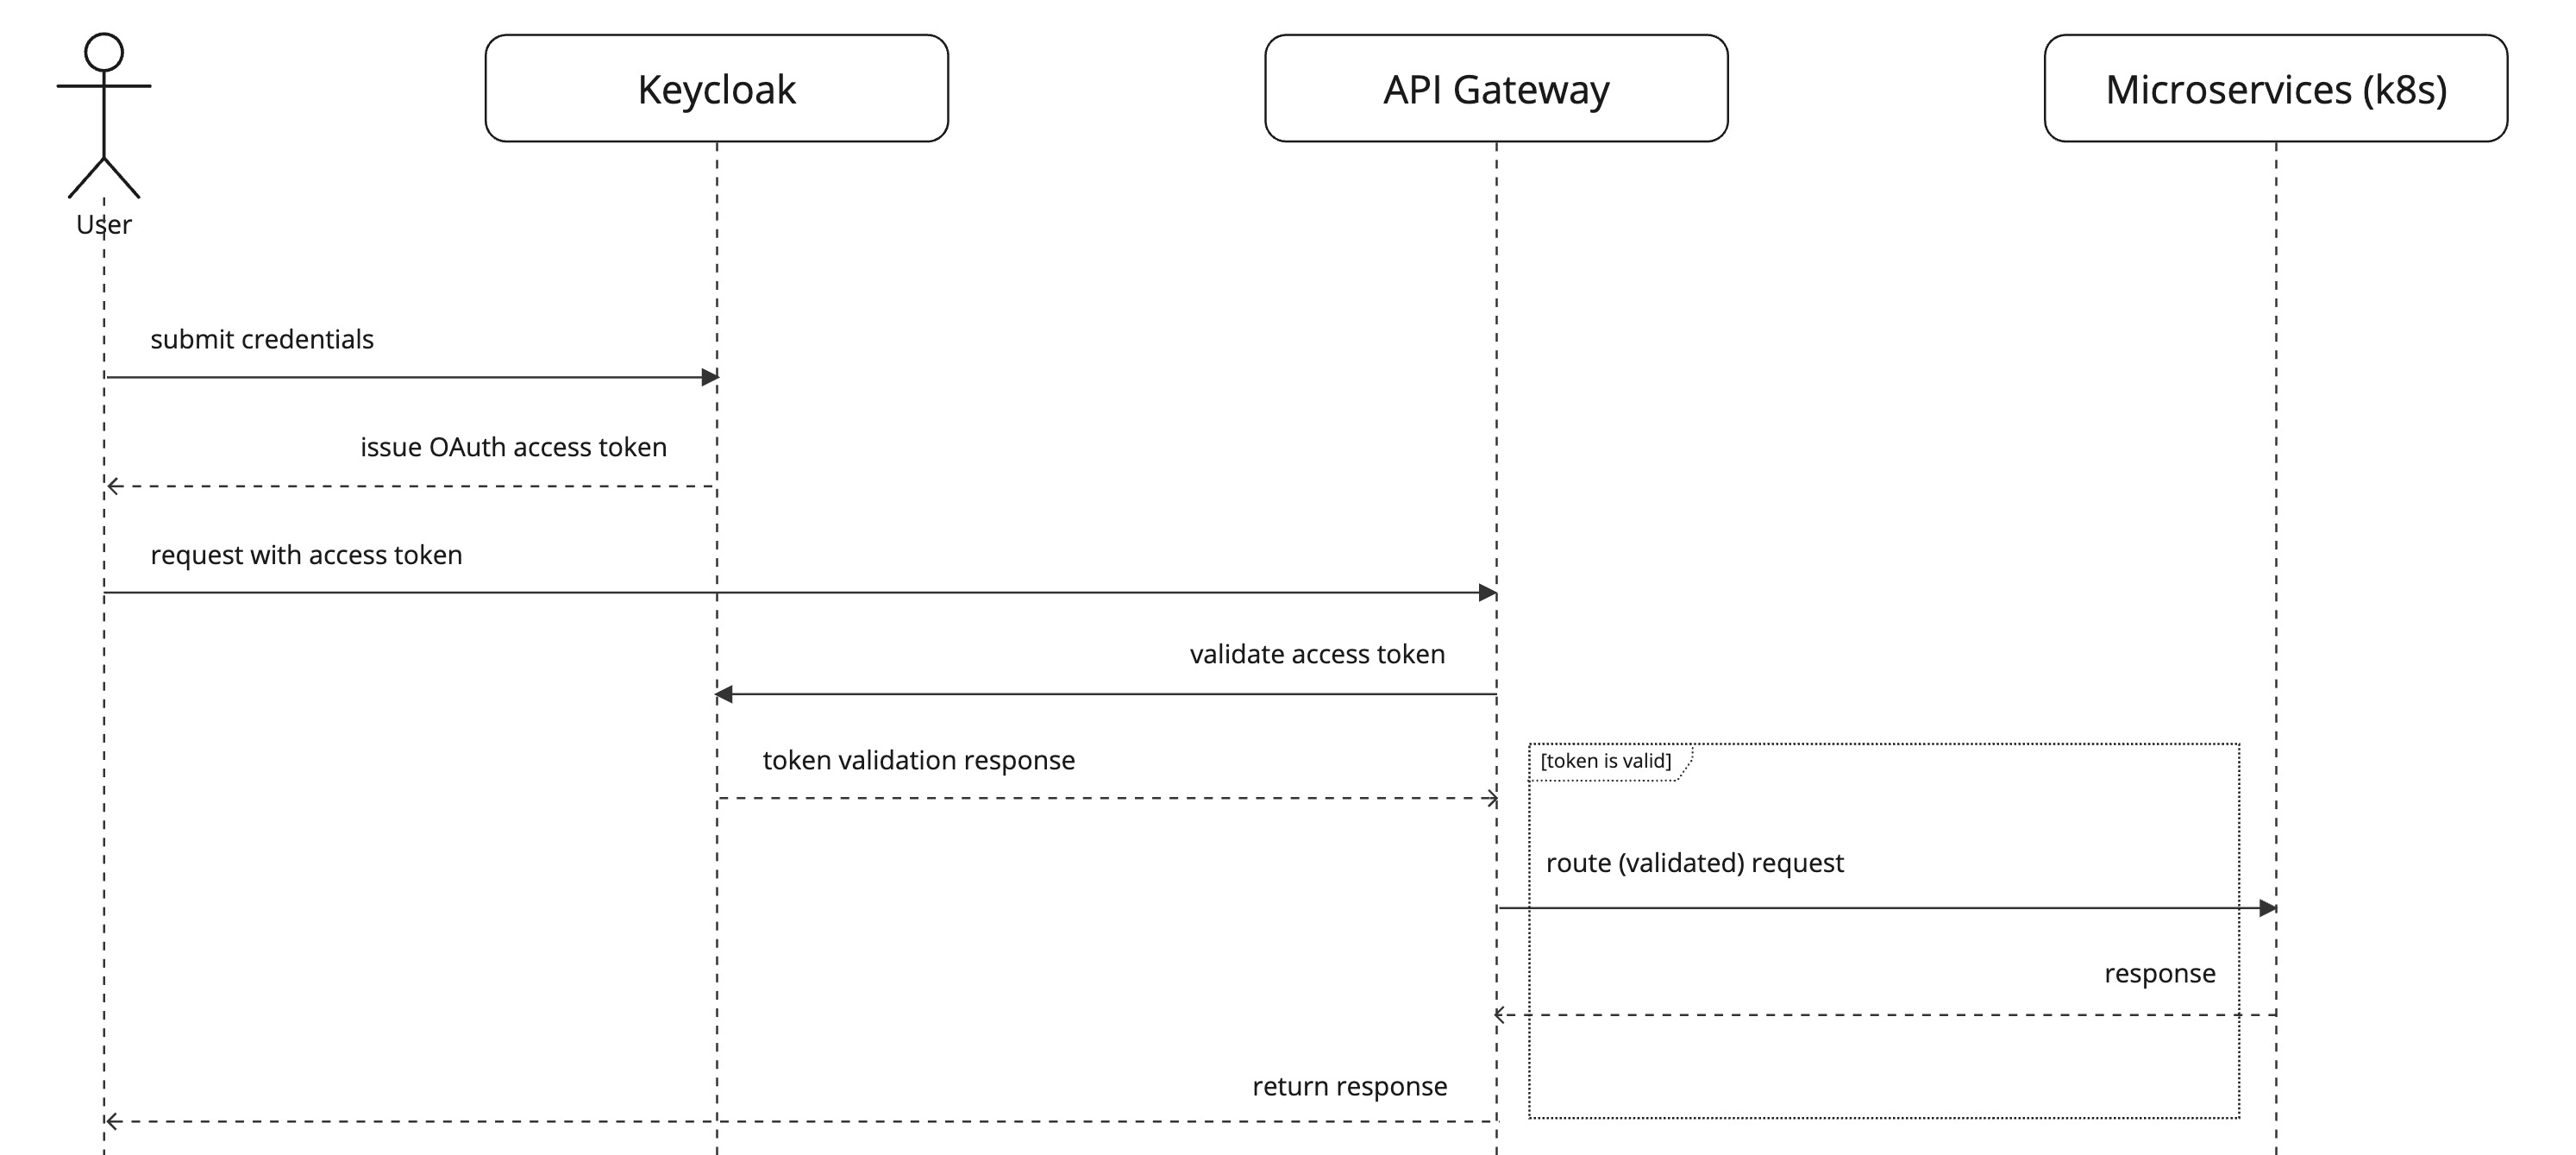
\includegraphics[width=1\textwidth]{Authentication.jpg}
    \caption{Authentication}
    \label{fig:auth-diagram}
\end{figure}

\begin{longtable}{|l|p{7.5cm}|}
\hline
\textbf{Term} & \textbf{Definition} \\ \hline
\endfirsthead
\textbf{User} & The end user providing credentials to access the system. \\ \hline
\textbf{Keycloak} & An external identity and access management service (Keycloak) providing OAuth-based authentication and token issuance. \\ \hline
\textbf{Access Token} & An OAuth token issued by Keycloak, granting temporary access to the API on behalf of the authenticated user. \\ \hline
\textbf{API Gateway} & A gateway responsible for validating OAuth access tokens and enforcing access controls. \\ \hline
\textbf{Microservices (k8s)} & Backend services accessed by users through the API Gateway, with resource permissions validated. \\ \hline
\end{longtable}
\newpage
\subsection{Centralized Logging and Metrics}

Centralized logging and metrics provide observability and performance tracking across the system. Logs are collected using Fluent Bit, aggregated via Kafka, indexed and stored in downstream systems, and visualized in Grafana. Metrics are scraped with Prometheus and also visualized in Grafana to correlate system behavior and performance.

\begin{enumerate}
    \item Logs are collected from microservices in a Kubernetes cluster using Fluent Bit and sent to Kafka for centralized aggregation.
    \item Metrics are scraped directly from services and Kafka using Prometheus.
    \item Downstream systems index and process the aggregated data.
    \item Grafana visualizes both logs and metrics on unified dashboards, enabling centralized monitoring and alerting.
\end{enumerate}

\begin{figure}[h!]
    \centering
    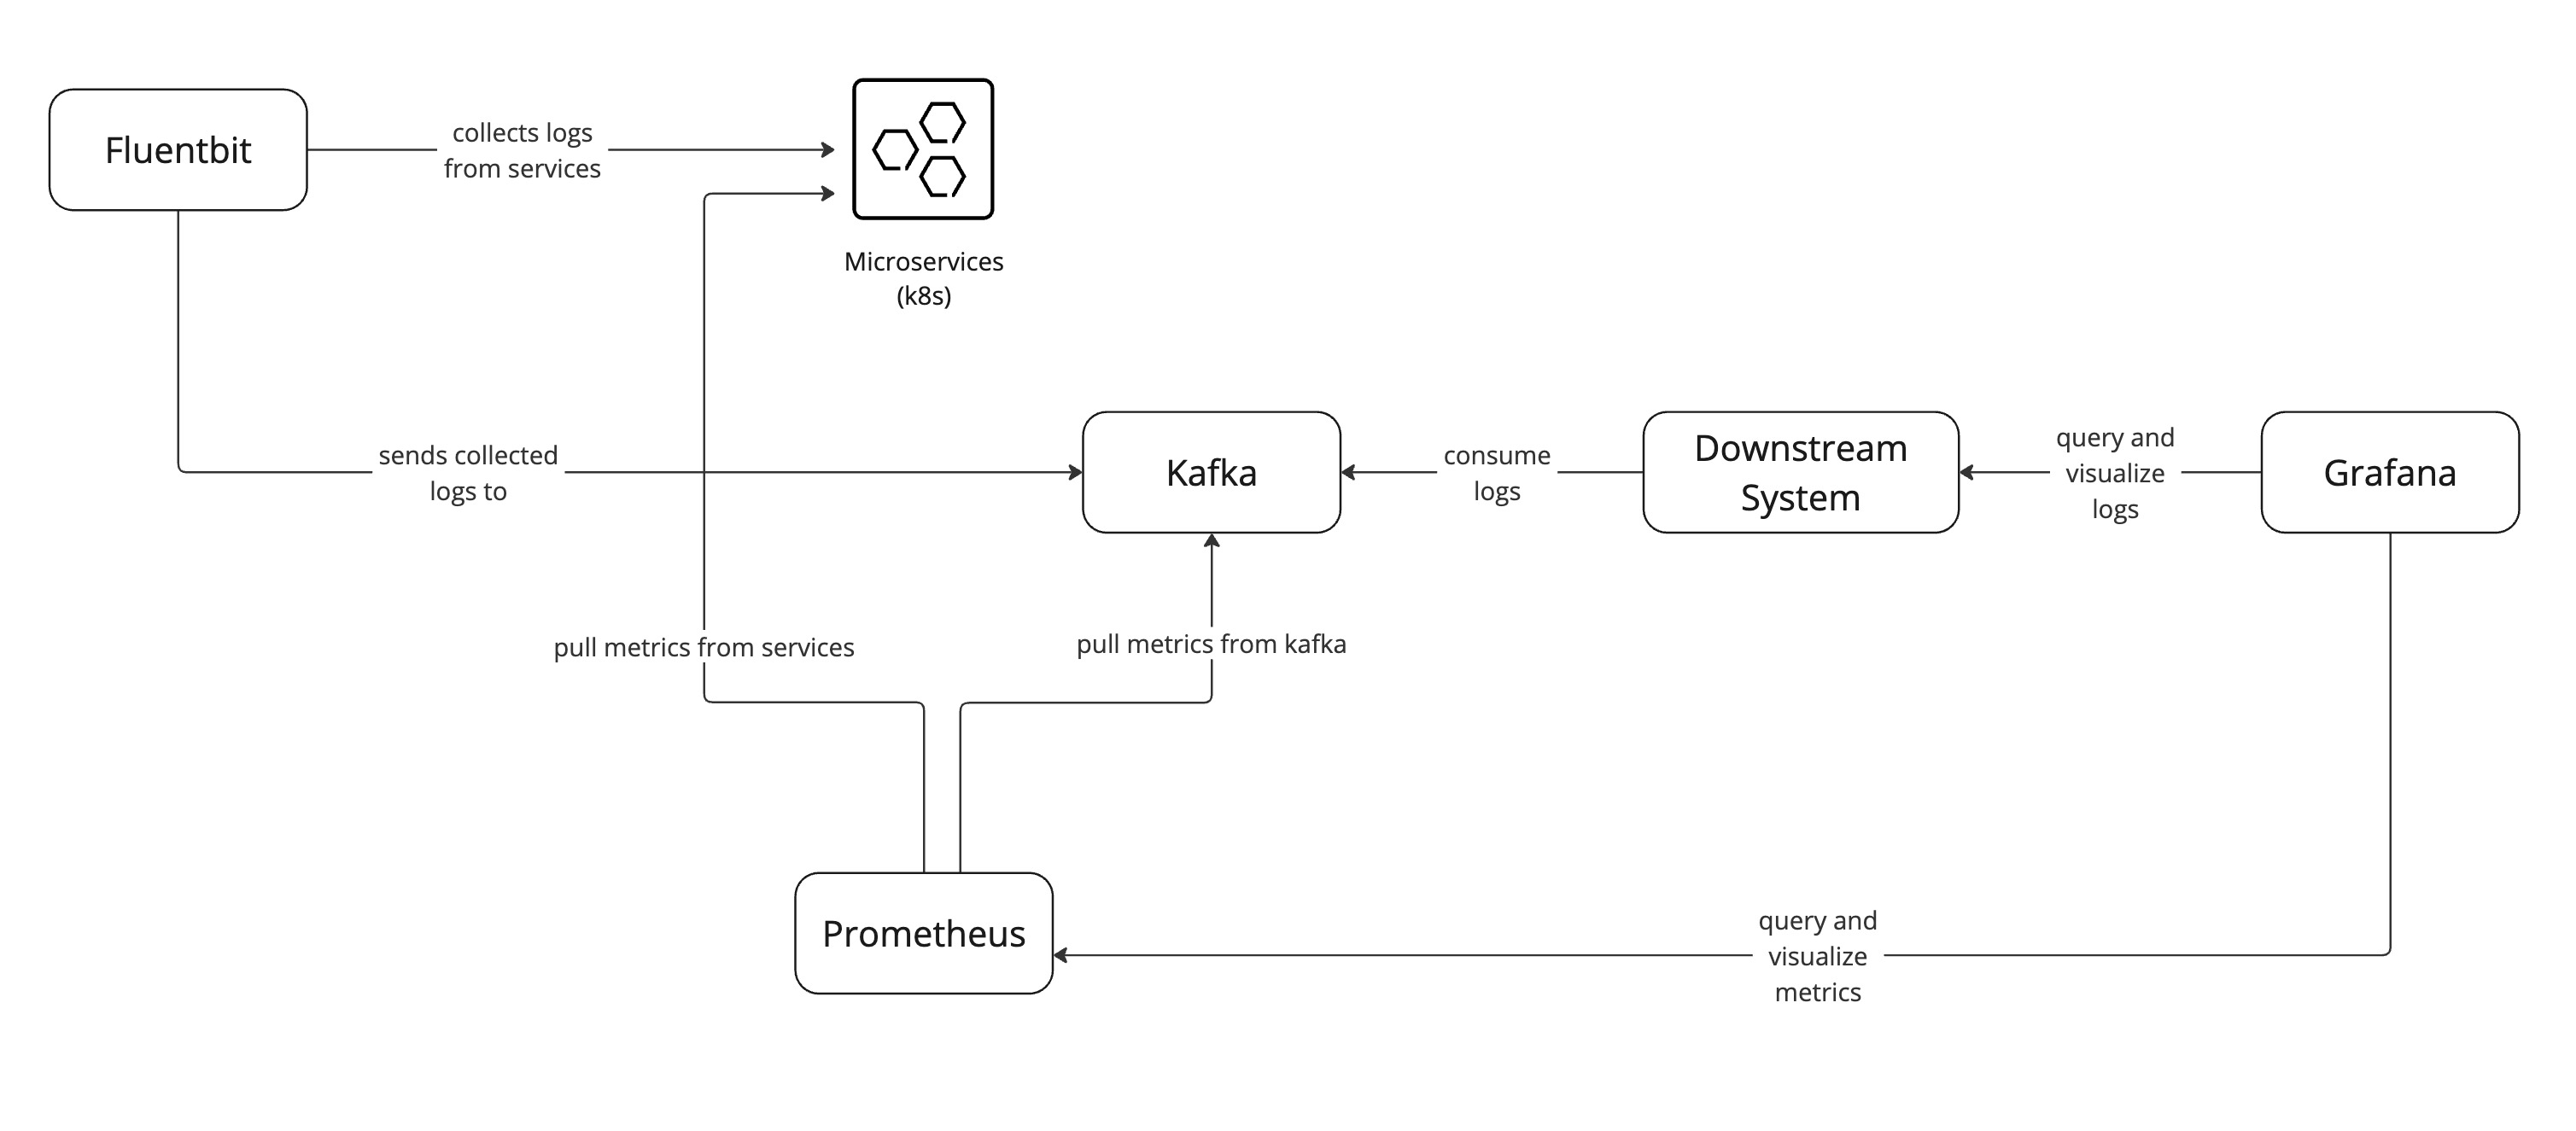
\includegraphics[width=1\textwidth]{Logging.jpg}
    \caption{Logging and Metrics}
    \label{fig:auth-diagram}
\end{figure}

\begin{longtable}{|l|p{7.5cm}|}
\hline
\textbf{Term} & \textbf{Definition} \\ \hline
\endfirsthead
\textbf{Microservices (k8s)} & Services running in a Kubernetes cluster, emitting logs and exposing metrics. \\ \hline
\textbf{Fluent Bit} & A lightweight log processor running as a DaemonSet in the cluster, collecting logs from pods/nodes. \\ \hline
\textbf{Kafka} & A distributed message broker used to aggregate logs and metrics for downstream processing. \\ \hline
\textbf{Prometheus} & A monitoring tool that scrapes metrics from the services and Kafka, storing and indexing them. \\ \hline
\textbf{Downstream System} & Systems (e.g., Loki or custom consumers) consuming data from Kafka for indexing or storage. \\ \hline
\textbf{Grafana} & A visualization tool querying Prometheus and other backends for centralized metrics and log dashboards. \\ \hline
\end{longtable}

\subsection{Stateless Communication}

Stateless communication ensures modularity by externalizing transient state management. Redis acts as a central hub for session data, player interactions, and real-time game updates, enabling microservices to remain stateless and focus on their core functions.

\begin{enumerate}
    \item Redis stores session data, player interactions, and game states, ensuring consistency and quick access across services.
    \item Redis Server enables efficient broadcasting of updates to WebSocket clients.
    \item WebSocket servers offload state to Redis, allowing any server instance to manage connections (horizontal scaling).
\end{enumerate}

\begin{figure}[h!]
    \centering
    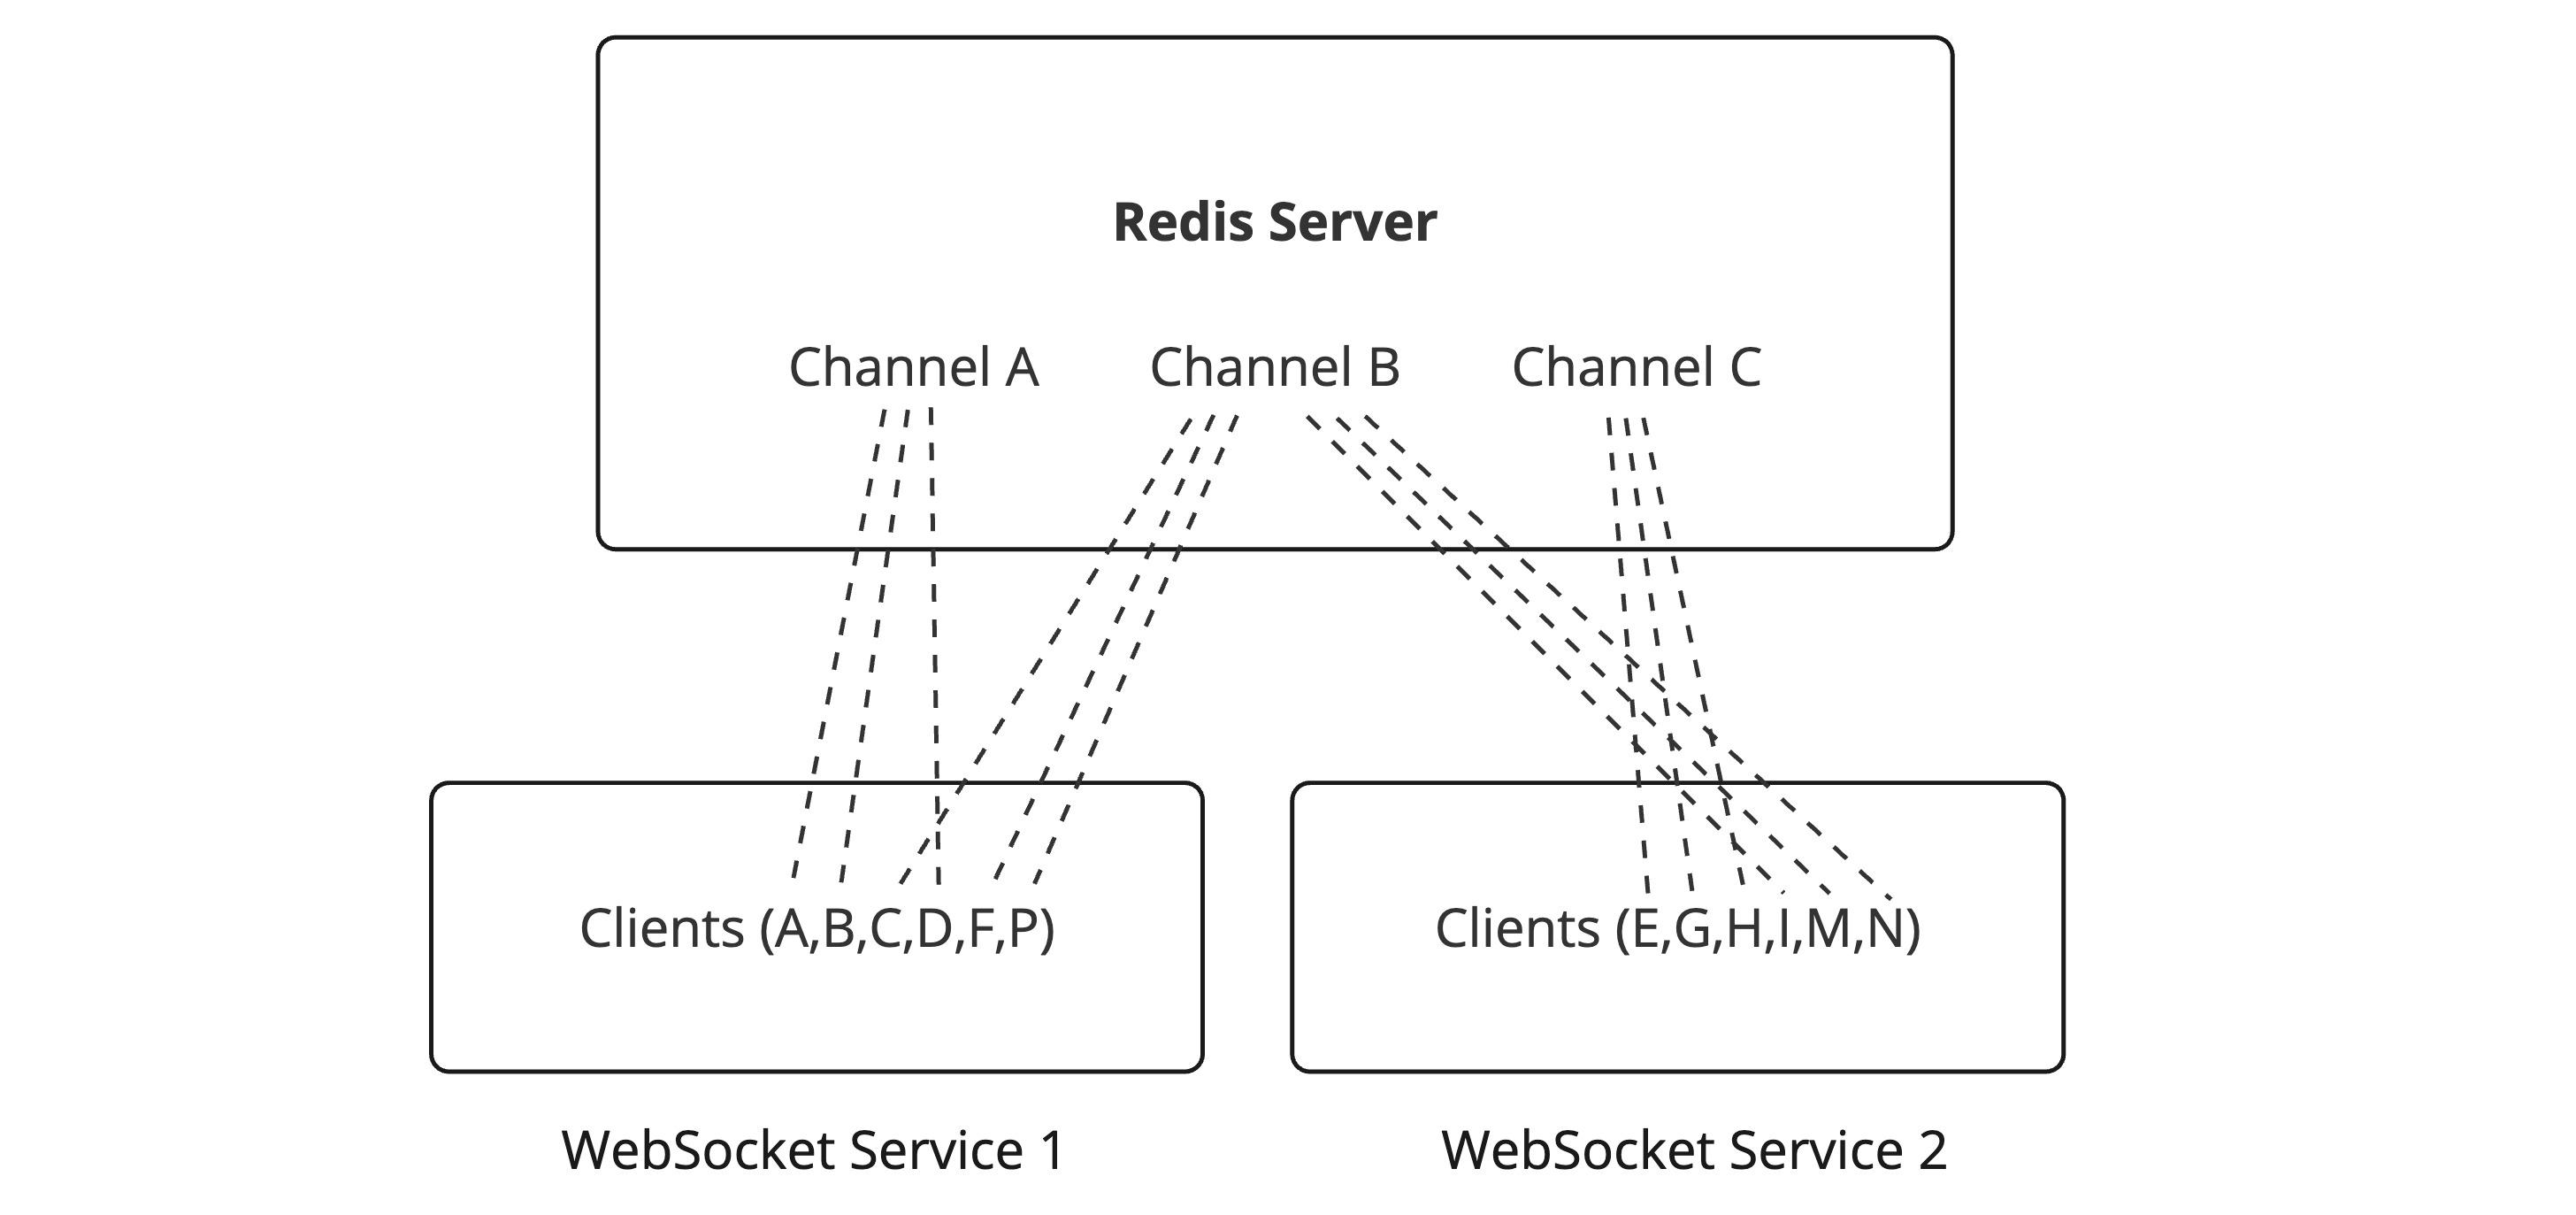
\includegraphics[width=1\textwidth]{Stateless.jpg}
    \caption{Stateless Communication}
    \label{fig:auth-diagram}
\end{figure}

\begin{longtable}{|p{4cm}|p{7.5cm}|}
\hline
\textbf{Term} & \textbf{Definition} \\ \hline
\endfirsthead
\textbf{Redis Server} & Acts as a central hub for transient state management and message broadcasting. It hosts channels (e.g., Channel A, B, C) to organize messages. \\ \hline
\textbf{Channel} & A logical topic in Redis Pub/Sub used to route messages to subscribed clients. Examples include:
\begin{itemize}
    \item \textbf{Channel A}: Broadcasts updates related to a specific escape room.
    \item \textbf{Channel B}: Manages leaderboard updates.
    \item \textbf{Channel C}: Handles general notifications.
\end{itemize} \\ \hline
\textbf{WebSocket Service} & A server instance (e.g., WebSocket Service 1 or 2) responsible for managing WebSocket connections. It receives and forwards messages between clients and the Redis Server. \\ \hline
\textbf{Client} & A connected WebSocket client (e.g., A, B, C on Service 1 or E, G, H on Service 2). Clients subscribe to one or more Redis channels to receive updates in real time. \\ \hline
\textbf{Pub/Sub (Publish/Subscribe)} & A messaging pattern used by Redis to broadcast messages to all subscribers of a specific channel. Clients on different WebSocket servers receive messages through this mechanism. \\ \hline
\end{longtable}